%{{第七十五回}}{第七十五回}}

\chapter{开夜宴异兆发悲音 赏中秋新词得佳谶}
{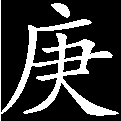
\includegraphics[width=3mm]{../Images/00004}\kaishu 乾隆二十一年五月初七日对清。◇缺中秋诗,俟雪芹。}

{\kaishu □□□ 开夜宴 发悲音}

{\kaishu □□□ 赏中秋 得佳谶}

{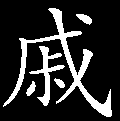
\includegraphics[width=3mm]{../Images/00005}\kaishu 贾珍居长,不能承先启后,丕震家风,兄弟问柳寻花,父子呼幺喝六,贾氏宗风,其坠地矣。安得不发先灵一叹!}

话说尤氏从惜春处赌气出来,正欲往王夫人处去。跟从的老嬷嬷们因悄悄的回道:``奶奶且别往上房去。才有甄家的几个人来,还有些东西,不知是作什么机密事。奶奶这一去恐不便。''尤氏听了道:``昨日听见你爷说,\elegantpar{看邸报甄家犯了罪}{报纸},现今抄没家私,调取进京治罪。怎么又有人来?''老嬷嬷道:``正是呢。才来了几个女人,气色不成气色,慌慌张张的,想必有什么瞒人的事情也是有的。''

尤氏听了,便不往前去,仍往李氏这边来了。{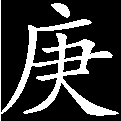
\includegraphics[width=3mm]{../Images/00004}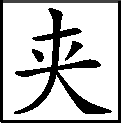
\includegraphics[width=3mm]{../Images/00012}\footnotesize \kaishu 前只有探春一语,过至此回又用尤氏略为陪点,且轻轻淡染出甄家事故,此画家{(来)}{[}谓{]}``落墨之法''也。}\href{../Text/part0079_split_000.html\#lnkback_1_a}{\textsuperscript{①}}恰好太医才诊了脉去。李纨近日也略觉精爽了些,拥衾欹\href{../Text/part0079_split_000.html\#lnkback_2_a}{\textsuperscript{②}}枕,坐在床上,正欲一二人来说些闲话。因见尤氏进来不似往日和蔼可亲,只呆呆的坐着。李纨因问道:``你过来了这半日,可在别屋里吃些东西没有?只怕饿了。''命素云瞧有什么新鲜点心拣了来。尤氏忙止道:``不必,不必。你这一向病着,那里有什么新鲜东西。况且我也不饿。''李纨道:``昨日他姨娘家送来的好茶面子,倒是对碗来你喝罢。''说毕,便吩咐人去对茶。尤氏出神无语。跟来的丫头媳妇们因问:``奶奶今日中晌尚未洗脸,这会子趁便可净一净好?''尤氏点头。李纨忙命素云来取自己的妆奁。素云一面取来,一面将自己的胭粉拿来,笑道:``我们奶奶就少这个。奶奶不嫌脏,这是我的,能着用些。''李纨道:``我虽没有,你就该往姑娘们那里取去。怎么公然拿出你的来。幸而是他,若是别人,岂不恼呢。''尤氏笑道:``这又何妨。自来我凡过来,谁的没使过,今日忽然又嫌脏了?''一面说,一面盘膝坐在炕沿上。银蝶上来忙代为卸去腕镯戒指,又将一大袱手巾盖在下截,将衣裳护严。小丫鬟\elegantpar{炒豆儿}{这名字}捧了一大盆温水走至尤氏跟前,只弯腰捧着。银蝶笑道:``说一个个没机变的,说一个葫芦就是一个瓢。奶奶不过待咱们宽些,在家里不管怎样罢了,你就得了意,不管在家出外,当着亲戚也只随着便了。''尤氏道:``你随他去罢,横竖洗了就完事了。''炒豆儿忙赶着跪下。尤氏笑道:``你们家下大小的人只会讲外面假礼假体面,究竟作出来的事都够使的了。''{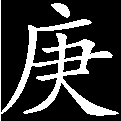
\includegraphics[width=3mm]{../Images/00004}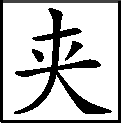
\includegraphics[width=3mm]{../Images/00012}\footnotesize \kaishu 按尤氏犯七出之条,不过只是``过于从夫''四字,此世间妇人之常情耳。其心术慈厚宽顺,竟可出于阿凤之上,特用此明犯七出之人从公一论,可知贾宅中暗犯七出之人亦不少。似明犯者反可宥恕,其饰己非而扬人恶者,阴昧僻谲之流,实不能容于世者也。◇此为打草惊蛇法,实写邢夫人也。}李纨听如此说,便知他已知道昨夜的事,因笑道:``你这话有因,谁作事究竟够使了?''尤氏道:``你倒问我!你敢是病着死过去了!''

一语未了,只见人报:``宝姑娘来了。''忙说快请时,宝钗已走进来。尤氏忙擦脸起身让坐,因问:``怎么一个人忽然走来,别的姊妹都怎么不见?''宝钗道:``正是我也没有见他们。只因今日我们奶奶身上不自在,家里两个女人也都因时症未起炕,别的靠不得,我今儿要出去伴着老人家夜里作伴儿。要去回老太太、太太,我想又不是什么大事,且不用提,等好了我横竖进来的,所以来告诉大嫂子一声。''李纨听说,只看着尤氏笑。尤氏也只看着李纨笑。一时尤氏盥沐已毕,大家吃面茶。李纨因笑道:``既这样,且打发人去请姨娘的安,问是何病。我也病着,不能亲自来的。好妹妹,你去只管去,我自打发人去到你那里去看屋子。你好歹住一两天还进来,别叫我落不是。''宝钗笑道:``落什么不是呢,这也是通共常情,你又不曾卖放了贼。依我的主意,也不必添人过去,竟把云丫头请了来,你和他住一两日,岂不省事。''尤氏道:``可是史大妹妹往那里去了?''宝钗道:``我才打发他们找你们探丫头去了,叫他同到这里来,我也明白告诉他。''

正说着,果然报:``云姑娘和三姑娘来了。''大家让坐已毕,宝钗便说要出去一事,探春道:``很好。不但姨妈好了还来的,就便好了不来也使得。''尤氏笑道:``这话奇怪,怎么撵起亲戚来了?''探春冷笑道:``正是呢,有叫人撵的,不如我先撵。亲戚们好,也不在必要死住着才好。咱们倒是一家子亲骨肉呢,一个个不像乌眼鸡,恨不得你吃了我,我吃了你!''尤氏忙笑道:``我今儿是那里来的晦气,偏都碰着你姊妹们的气头儿上了。''探春道:``谁叫你赶热灶来了!''因问:``谁又得罪了你呢?''因又寻思道:``惜丫头不犯罗唣你,却是谁呢?''尤氏只含糊答应。探春知他畏事不肯多言,因笑道:``你别装老实了。除了朝廷治罪,没有砍头的,你不必畏头畏尾。实告诉你罢,我昨日把王善保家那老婆子打了,我还顶着个罪呢。不过背地里说我些闲话,难道他还打我一顿不成!''宝钗忙问因何又打他,探春悉把昨夜怎的抄检,怎的打他,一一说了出来。尤氏见探春已经说了出来,便把惜春方才之事也说了出来。探春道:``这是他的僻性,孤介太过,我们再傲不过他的。''又告诉他们说:``今日一早不见动静,打听凤辣子又病了。我就打发我妈妈出去打听王善保家的是怎样。回来告诉我说,王善保家的挨了一顿打,大太太嗔着他多事。''尤氏李纨道:``这倒也是正理。''探春冷笑道:``这种掩饰谁不会作,且再瞧就是了。''尤氏李纨皆默无所答。一时估着前头用饭,湘云和宝钗回房打点衣衫,不在话下。

尤氏等遂辞了李纨,往贾母这边来。贾母歪在榻上,王夫人说甄家因何获罪,如今抄没了家产,回京治罪等语。贾母听了正不自在,恰好见他姊妹来了,因问从那里来的?可知凤姐妯娌两个的病今日怎样?尤氏等忙回道:``今日都好些。''贾母点头叹道:``咱们别管人家的事,且商量咱们八月十五日赏月是正经。''{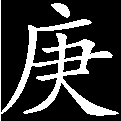
\includegraphics[width=3mm]{../Images/00004}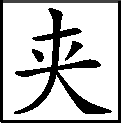
\includegraphics[width=3mm]{../Images/00012}\footnotesize \kaishu 贾母已看破狐悲兔死,故不改{(已)}{[}色{]},聊{(未)}{[}为{]}自遣耳。}王夫人笑道:``都已预备下了。不知老太太拣那里好,只是园里空,夜晚风冷。''贾母笑道:``多穿两件衣服何妨,那里正是赏月的地方,岂可倒不去的。''

说话之间,早有媳妇丫鬟们抬过饭桌来,王夫人尤氏等忙上来放箸捧饭。贾母见自己的几色菜已摆完,另有两大捧盒内捧了几色菜来,便知是各房另外孝敬的旧规矩。贾母因问:``都是些什么?上几次我就吩咐,如今可以把这些蠲了罢,你们还不听。如今比不得在先辐辏的时光了。''鸳鸯忙道:``我说过几次,都不听,也只罢了。''王夫人笑道:``不过都是家常东西。今日我吃斋没有别的。\elegantpar{那些面筋豆腐老太太又不大甚爱吃,只拣了一样椒油莼齑酱来。}{倒爱吃}''贾母笑道:``这样正好,正想这个吃。''鸳鸯听说,便将碟子挪在跟前。宝琴一一的让了,方归坐。贾母便命探春来同吃。探春也都让过了,便和宝琴对面坐下。待书忙去取了碗来。鸳鸯又指那几样菜道:``这两样看不出是什么东西来,大老爷送来的。这一碗是鸡髓笋,是外头老爷送上来的。''一面说,一面就只将这碗笋送至桌上。贾母略尝了两点,便命:``将那两样着人送回去,就说我吃了。以后不必天天送,我想吃自然来要。''媳妇们答应着,仍送过去,不在话下。

贾母因问:``有稀饭吃些罢了。''尤氏早捧过一碗来,说是红稻米粥。贾母接来吃了半碗,便吩咐:``将这粥送给凤哥儿吃去,''又指着``这一碗笋和这一盘风腌果子狸给颦儿宝玉两个吃去,那一碗肉给兰小子吃去。''又向尤氏道:``我吃了,你就来吃了罢。''尤氏答应,待贾母漱口洗手毕,贾母便下地和王夫人说闲话行食。尤氏告坐。探春宝琴二人也起来了,笑道:``失陪,失陪。''尤氏笑道:``剩我一个人,大排桌的吃不惯。''贾母笑道:``鸳鸯琥珀来趁势也吃些,又作了陪客。''尤氏笑道:``好,好,好,我正要说呢。''贾母笑道:``看着多多的人吃饭,最有趣的。''又指银蝶道:``这孩子也好,也来同你主子一块来吃,等你们离了我,再立规矩去。''尤氏道:``快过来,不必装假。''贾母负手看着取乐。因见伺候添饭的人手内捧着一碗下人的米饭,尤氏吃的仍是白粳米饭,贾母问道:``你怎么昏了,盛这个饭来给你奶奶。''那人道:``老太太的饭吃完了。今日添了一位姑娘,所以短了些。''鸳鸯道:``{如今都是可着头做帽子了,要一点儿富馀也不能的。}{天时气运}''王夫人忙回道:``这一二年旱涝不定,田上的米都不能按数交的。这几样细米更艰难了,所以都可着吃的多少关去,生恐一时短了,买的不顺口。''贾母笑道:``这正是`巧媳妇做不出没米的粥'来。''众人都笑起来。鸳鸯道:``既这样,你就去把三姑娘的饭拿来添也是一样,就这样笨。''尤氏笑道:``我这个就够了,也不用取去。''鸳鸯道:``你够了,我不会吃的。''地下的媳妇们听说,方忙着取去了。{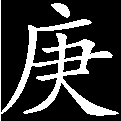
\includegraphics[width=3mm]{../Images/00004}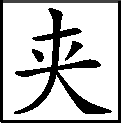
\includegraphics[width=3mm]{../Images/00012}\footnotesize \kaishu 总伏下文。}一时王夫人也去用饭。

这里尤氏直陪贾母说话取笑。到起更的时候,贾母说:``黑了,过去罢。''尤氏方告辞出来。走至大门前上了车,银蝶坐在车沿上。众媳妇放下帘子来,便带着小丫头们先直走过那边大门口等着去了。因二府之门相隔没有一箭之路,每日家常来往不必定要周备,况天黑夜晚之间回来的遭数更多,所以老嬷嬷带着小丫头,只几步便走了过来。两边大门上的人都到东西街口,早把行人断住。尤氏大车上也不用牲口,只用七八个小厮挽环拽轮,轻轻的便推拽过这边阶矶上来。于是众小厮退过狮子以外,众嬷嬷打起帘子,银蝶先下来,然后搀下尤氏来。大小七八个灯笼照的十分真切。尤氏因见两边狮子下放着四五辆大车,便知系来赴赌之人所乘,遂向银蝶众人道:``你看,坐车的是这样,骑马的还不知有几个呢。马自然在圈里拴着,咱们看不见。也不知道他娘老子挣下多少钱与他们,这么开心儿。''一面说,一面已到了厅上。贾蓉之妻带领家下媳妇丫头们,也都秉烛接了出来。尤氏笑道:``成日家我要偷着瞧瞧他们,也没得便。今儿倒巧,就顺便打他们窗户跟前走过去。''众媳妇答应着,提灯引路,又有一个先去悄悄的知会伏侍的小厮们不要失惊打怪。于是尤氏一行人悄悄的来至窗下,只听里面称三赞四,耍笑之音虽多,{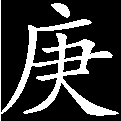
\includegraphics[width=3mm]{../Images/00004}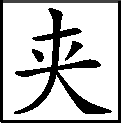
\includegraphics[width=3mm]{../Images/00012}\footnotesize \kaishu 妙!先画赢家。}又兼有恨五骂六,忿怨之声亦不少。{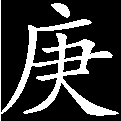
\includegraphics[width=3mm]{../Images/00004}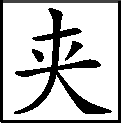
\includegraphics[width=3mm]{../Images/00012}\footnotesize \kaishu 妙!又画输家。}

原来贾珍近因居丧,每不得游玩旷朗,又不得观优闻乐作遣。无聊之极,便生了个破闷之法。日间以习射为由,请了各世家弟兄及诸富贵亲友来较射。因说:``白白的只管乱射,终无裨益,不但不能长进,而且坏了式样,必须立个罚约,赌个利物,大家才有勉力之心。''因此在\elegantpar{天香楼}{楼}下箭道内立了鹄子,皆约定每日早饭后来射鹄子。贾珍不肯出名,便命贾蓉作局家。这些来的皆系世袭公子,人人家道丰富,且都在少年,正是斗鸡走狗,问柳评花的一干游荡纨绔。因此大家议定,每日轮流作晚饭之主,------每日来射,不便独扰贾蓉一人之意。于是天天宰猪割羊,屠鹅戮鸭,好似临潼斗宝一般,都要卖弄自己家的好厨役好烹炮。不到半月工夫,贾赦贾政听见这般,不知就里,反说这才是正理,文既误矣,武事当亦该习,况在武荫之属。两处遂也命贾环、贾琮、宝玉、贾兰等四人于饭后过来,跟着贾珍习射一回,方许回去。

贾珍志不在此,再过一二日便渐次以歇臂养力为由,晚间或抹抹骨牌,赌个酒东而已,至后渐次至钱。如今三四月的光景,竟一日一日赌胜于射了,公然斗叶掷骰,放头开局,夜赌起来。家下人借此各有些进益,巴不得的如此,所以竟成了势了。外人皆不知一字。近日邢夫人之胞弟邢德全也酷好如此,故也在其中。又有薛蟠,\elegantpar{头一个惯喜送钱与人的}{头一个,头一个},见此岂不快乐。邢德全虽系邢夫人之胞弟,却居心行事大不相同。这个邢德全只知吃酒赌钱,眠花宿柳为乐,手中滥漫使钱,待人无二心,好酒者喜之,不饮者则不去亲近,无论上下主仆皆出自一意,并无贵贱之分,因此都唤他``傻大舅''。薛蟠是早已出名的呆大爷。今日二人皆凑在一处,都爱``抢新快''爽利,便又会了两家,在外间炕上``抢新快''。别的又有几家在当地下大桌上打公番。里间又一起斯文些的,抹骨牌打天九。此间伏侍的小厮都是十五岁以下的孩子,若成丁的男子到不了这里,故尤氏方潜至窗外偷看。其中有两个十六七岁娈童以备奉酒的,都打扮的粉妆玉琢。

今日薛蟠又输了一张,正没好气,幸而掷第二张完了,算来除翻过来倒反赢了,心中只是兴头起来。贾珍道:``且打住,吃了东西再来。''因问那两处怎样。里头打天九的,也作了账等吃饭。打公番的未清,且不肯吃。于是各不能顾,先摆下一大桌,贾珍陪着吃,命贾蓉落后陪那一起。薛蟠兴头了,便搂着一个娈童吃酒,又命将酒去敬邢傻舅。傻舅输家,没心绪,吃了两碗,便有些醉意,嗔着两个娈童只赶着赢家不理输家了,因骂道:``你们这起兔子,就是这样专洑上水。天天在一处,谁的恩你们不沾,只不过我这一会子输了几两银子,你们就三六九等了。难道从此以后再没有求着我们的事了!''众人见他带酒,忙说:``很是,很是。果然他们风俗不好。''因喝命:``快敬酒赔罪。''两个娈童都是演就的局套,忙都跪下奉酒,说:``我们这行人,师父教的不论远近厚薄,只看一时有钱有势就亲敬,便是活佛神仙,一时没了钱势了,也不许去理他。况且我们又年轻,又居这个行次,求舅太爷体恕些我们就过去了。''{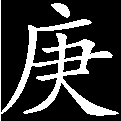
\includegraphics[width=3mm]{../Images/00004}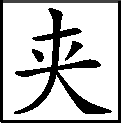
\includegraphics[width=3mm]{../Images/00012}\footnotesize \kaishu 调侃,骂死世人。不是骂。 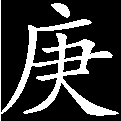
\includegraphics[width=3mm]{../Images/00004}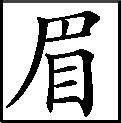
\includegraphics[width=3mm]{../Images/00010}\footnotesize \kaishu 此一段娈童语句太真,反不得其为钱为势之神,当改以委曲认罪语方妥。}\href{../Text/part0079_split_000.html\#lnkback_3_a}{\textsuperscript{③}}说着,便举着酒俯膝跪下。邢大舅心内虽软了,只还故作怒意不理。众人又劝道:``这孩子是实情话。老舅是久惯怜香惜玉的,如何今日反这样起来?若不吃这酒,他两个怎样起来。''邢大舅已撑不住了,便说道:``若不是众位说,我再不理。''说着,方接过来一气喝干了。又斟一碗来。

这邢大舅便酒勾往事,醉露真情起来,乃拍案对贾珍叹道:``怨不的他们视钱如命。多少世宦大家出身的,若提起`钱势'二字,连骨肉都不认了。老贤甥,昨日我和你那边的令伯母赌气,你可知道否?''贾珍道:``不曾听见。''邢大舅叹道:``就为钱这件混帐东西。利害,利害!''贾珍深知他与邢夫人不睦,每遭邢夫人弃恶,扳出怨言,因劝道:``老舅,你也太散漫些。若只管花去,有多少给老舅花的。''邢大舅道:``老贤甥,你不知我邢家底里。我母亲去世时我尚小,世事不知。他姊妹三个人,只有你令伯母年长出阁,一分家私都是他把持带来。如今二家姐虽也出阁,他家也甚艰窘,三家姐尚在家里,一应用度都是这里陪房王善保家的掌管。我便来要钱,也非要的是你贾府的,我邢家家私也就够我花了。无奈竟不得到手,所以有冤无处诉。''{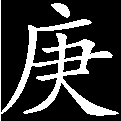
\includegraphics[width=3mm]{../Images/00004}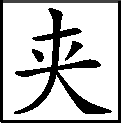
\includegraphics[width=3mm]{../Images/00012}\footnotesize \kaishu ``众恶之,必察也。''今邢夫人一人,贾母先恶之,恐贾母心偏,亦可解之。若贾琏阿凤之怨,恐儿女之私,亦可解之。若探春之怒,{[}恐{]}女子不识大而知小,亦可解之。今又忽用乃弟一怨,吾不知将又何如矣。}贾珍见他酒后叨叨,恐人听见不雅,连忙用话解劝。

外面尤氏听得十分真切,乃悄向银蝶笑道:``你听见了?这是北院里大太太的兄弟抱怨他呢。可怜他亲兄弟还是这样说,这就怨不得这些人了。''因还要听时,正值打公番者也歇住了,要吃酒。因有一个问道:``方才是谁得罪了老舅,我们竟不曾听明白,且告诉我们评评理。''邢德全见问,便把两个娈童不理输的只赶赢的话说了一遍。这一个年少的纨绔道:``这样说,原可恼的,怨不得舅太爷生气。我且问你两个:舅太爷虽然输了,输的不过是银子钱,并没有输丢了鸡巴,怎就不理他了?''说着,众人大笑起来,连邢德全也喷了一地饭。尤氏在外面悄悄的啐了一口,骂道:``你听听,这一起子没廉耻的小挨刀的,才丢了脑袋骨子,就胡唚嚼毛了。再肏攮下黄汤去,还不知唚出些什么来呢。''一面说,一面便进去卸妆安歇。至四更时,贾珍方散,往配凤房里去了。

次日起来,就有人回西瓜月饼都全了,只待分派送人。贾珍吩咐配凤道:``你请你奶奶看着送罢,我还有别的事呢。''配凤答应去了,回了尤氏,尤氏只得一一分派遣人送去。一时配凤又来说:``爷问奶奶,今儿出门不出?说咱们是孝家,明儿十五过不得节,今儿晚上倒好,可以大家应个景儿,吃些瓜饼酒。''尤氏道:``我倒不愿出门呢。那边珠大奶奶又病了,凤丫头又睡倒了,我再不过去,越发没个人了。况且又不得闲,应什么景儿。''配凤道:``爷说了,今儿已辞了众人,直等十六才来呢,好歹定要请奶奶吃酒的。''尤氏笑道:``请我,我没的还席。''配凤笑着去了,一时又来笑道:``爷说,连晚饭也请奶奶吃,好歹早些回来,叫我跟了奶奶去呢。''尤氏道:``这样,早饭吃什么?快些吃了,我好走。''配凤道:``爷说早饭在外头吃,请奶奶自己吃罢。''尤氏问道:``今日外头有谁?''配凤道:``听见说外头有两个南京新来的,倒不知是谁。''说话之间,贾蓉之妻也梳妆了来见过。少时摆上饭来,尤氏在上,贾蓉之妻在下相陪,婆媳二人吃毕饭。尤氏便换了衣服,仍过荣府来,至晚方回去。

果然贾珍煮了一口猪,烧了一腔羊,馀者桌菜及果品之类,不可胜记,就在会芳园丛绿堂中,屏开孔雀,褥设芙蓉,带领妻子姬妾,先饭后酒,开怀赏月作乐。将一更时分,真是风清月朗,上下如银。贾珍因要行令,尤氏便叫配凤等四个人也都入席,下面一溜坐下,猜枚划拳,饮了一回。贾珍有了几分酒,益发高兴,便命取了一竿紫竹箫来,命配凤吹箫,文{{(化)}}{[}鸳{]}唱曲,喉清嗓嫩,真令人魄醉魂飞。唱罢复又行令。那天将有三更时分,贾珍酒已八分。大家正添衣饮茶,换盏更酌之际,忽听那边墙下有人长叹之声。大家明明听见,都悚然疑畏起来。{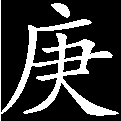
\includegraphics[width=3mm]{../Images/00004}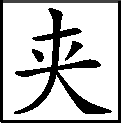
\includegraphics[width=3mm]{../Images/00012}\footnotesize \kaishu 余亦悚然疑畏。}贾珍忙厉声叱吒,问:``谁在那里?''连问几声,没有人答应。尤氏道:``必是墙外边家里人也未可知。''贾珍道:``胡说。这墙四面皆无下人的房子,况且那边又紧靠着祠堂,{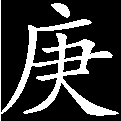
\includegraphics[width=3mm]{../Images/00004}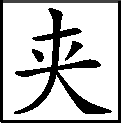
\includegraphics[width=3mm]{../Images/00012}\footnotesize \kaishu 奇绝神想,余更为之悚惧矣。}焉得有人。''一语未了,只听得一阵风声,竟过墙去了。恍惚闻得祠堂内槅扇开阖之声。只觉得风气森森,比先更觉凉飒起来,月色惨淡,也不似先明朗。众人都觉毛发倒竖。贾珍酒已醒了一半,只比别人撑持得住些,心下也十分疑畏,便大没兴头起来。勉强又坐了一会子,就归房安歇去了。次日一早起来,乃是十五日,带领众子侄开祠堂行朔望之礼,细察祠内,都仍是照旧好好的,并无怪异之迹。贾珍自为醉后自怪,也不提此事。礼毕,仍闭上门,看着锁禁起来。{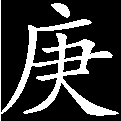
\includegraphics[width=3mm]{../Images/00004}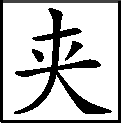
\includegraphics[width=3mm]{../Images/00012}\footnotesize \kaishu 未写荣府庆中秋,却先写宁府开夜宴,未写荣府数尽,先写宁府异兆。盖宁乃家宅,凡有关于吉凶者,故必先示之。且列祖祠{[}在{]}此,岂无得而警乎?凡人先人虽远,然气运相关,必有之理也。非宁府之祖独有感应也。}

贾珍夫妻至晚饭后方过荣府来。只见贾赦贾政都在贾母房内坐着说闲话,与贾母取笑。贾琏、宝玉、贾环、贾兰皆在地下侍立。贾珍来了,都一一见过。说了两句话后,贾母命坐,贾珍方在近门小杌子上告了坐,警身侧坐。贾母笑问道:``这两日你宝兄弟的箭如何了?''贾珍忙起身笑道:``大长进了,不但样式好,而且弓也长了一个力气。''贾母道:``这也够了,且别贪力,仔细努伤。''贾珍忙答应几个``是''。贾母又道:``你昨日送来的月饼好,西瓜看着好,打开却也罢了。''贾珍笑道:``月饼是新来的一个专做点心的厨子,我试了试果然好,才敢做了孝敬。西瓜往年都还可以,不知今年怎么就不好了。''贾政道:``大约今年雨水太勤之故。''贾母笑道:``此时月已上了,咱们且去上香。''说着,便起身扶着宝玉的肩,带领众人齐往园中来。

当下园之正门俱已大开,吊着羊角大灯。嘉荫堂前月台上,焚着斗香,秉着风烛,陈献着瓜饼及各色果品。邢夫人等一干女客皆在里面久候。真是月明灯彩,人气香烟,晶艳氤氲,不可形状。地下铺着拜毯锦褥。贾母盥手上香拜毕,于是大家皆拜过。贾母便说:``赏月在山上最好。''因命在那山脊上的大厅上去。众人听说,就忙着在那里去铺设。贾母且在嘉荫堂中吃茶少歇,说些闲话。一时,人回:``都齐备了。''贾母方扶着人上山来。王夫人等因说:``恐石上苔滑,还是坐竹椅上去。''贾母道:``天天有人打扫,况且极平稳的宽路,何必不疏散疏散筋骨。''于是贾赦贾政等在前导引,又是两个老婆子秉着两把羊角手罩,鸳鸯、琥珀、尤氏等贴身搀扶,邢夫人等在后围随,从下逶迤而上,不过百馀步,至山之峰脊上,便是这座敞厅。因在山之高脊,故名曰凸碧山庄。于厅前平台上列下桌椅,又用一架大围屏隔作两间。凡桌椅形式皆是圆的,特取团圆之意。上面居中贾母坐下,左垂首贾赦、贾珍、贾琏、贾蓉,右垂首贾政、宝玉、贾环、贾兰,团团围坐。只坐了半壁,下面还有半壁馀空。贾母笑道:``常日倒还不觉人少,今日看来,还是咱们的人也甚少,算不得甚么。{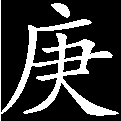
\includegraphics[width=3mm]{../Images/00004}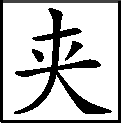
\includegraphics[width=3mm]{../Images/00012}\footnotesize \kaishu 未饮先感人丁,总是将散之兆。}想当年过的日子,到今夜男女三四十个,何等热闹。今日就这样,太少了。待要再叫几个来,他们都是有父母的,家里去应景,不好来的。如今叫女孩们来坐那边罢。''于是令人向围屏后邢夫人等席上将迎春,探春,惜春三个请出来。贾琏宝玉等一齐出坐,先尽他姊妹坐了,然后在下方依次坐定。

贾母便命折一枝桂花来,命一媳妇在屏后击鼓传花。若花到谁手中,饮酒一杯,罚说笑话一个。{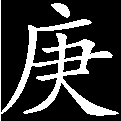
\includegraphics[width=3mm]{../Images/00004}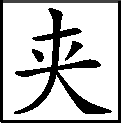
\includegraphics[width=3mm]{../Images/00012}\footnotesize \kaishu 不犯前几次饮酒。}于是先从贾母起,次贾赦,一一接过。鼓声两转,恰恰在贾政手中住了,{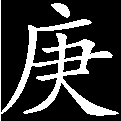
\includegraphics[width=3mm]{../Images/00004}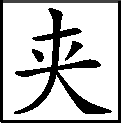
\includegraphics[width=3mm]{../Images/00012}\footnotesize \kaishu 奇妙!偏在政老手中,竟能使政老一谑,真大文章矣。}只得饮了酒。众姊妹弟兄皆你悄悄的扯我一下,我暗暗的又捏你一把,都含笑倒要听是何笑话。{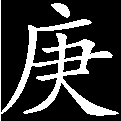
\includegraphics[width=3mm]{../Images/00004}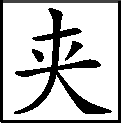
\includegraphics[width=3mm]{../Images/00012}\footnotesize \kaishu 余也要细听。}贾政见贾母喜悦,只得承欢。方欲说时,贾母又笑道:``若说的不笑了,还要罚。''贾政笑道:``只得一个,说来不笑,也只好受罚了。''因笑道:``一家子一个人最怕老婆的。''才说了一句,大家都笑了。因从不曾见贾政说过笑话,所以才笑。{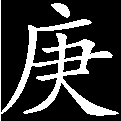
\includegraphics[width=3mm]{../Images/00004}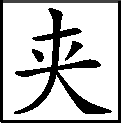
\includegraphics[width=3mm]{../Images/00012}\footnotesize \kaishu 是极,摹神之至。}贾母笑道:``这必是好的。''贾政笑道:``若好,老太太多吃一杯。''贾母笑道:``自然。''贾政又说道:``这个怕老婆的人从不敢多走一步。偏是那日是八月十五,到街上买东西,便遇见了几个朋友,死活拉到家里去吃酒。不想吃醉了,便在朋友家睡着了,第二日才醒,后悔不及,只得来家赔罪。他老婆正洗脚,说:`既是这样,你替我舔舔就饶你。'这男人只得给他舔,未免恶心要吐。他老婆便恼了,要打,说:`你这样轻狂!'唬得他男人忙跪下求说:`并不是\elegantpar{奶奶的脚脏}{阿Q}。只因昨晚吃多了黄酒,又吃了几块月饼馅子,所以今日有些作酸呢。'''说的贾母与众人都笑了。{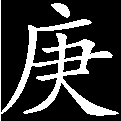
\includegraphics[width=3mm]{../Images/00004}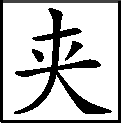
\includegraphics[width=3mm]{../Images/00012}\footnotesize \kaishu 这方是贾政之谑,亦善谑矣。}贾政忙斟了一杯,送与贾母。贾母笑道:``既这样,快叫人取烧酒来,别叫你们受累。''众人又都笑起来。

于是又击鼓,便从贾政传起,可巧传至宝玉鼓止。宝玉因贾政在坐,自是踧踖不安,花偏又在他手内,因想:``说笑话倘或不发笑,又说没口才,连一笑话不能说,何况别的,这有不是。若说好了,又说正经的不会,只惯油嘴贫舌,更有不是。不如不说的好。''{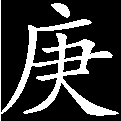
\includegraphics[width=3mm]{../Images/00004}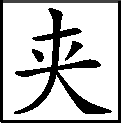
\includegraphics[width=3mm]{../Images/00012}\footnotesize \kaishu 实写旧日往事。}乃起身辞道:``我不能说笑话,求再限别的罢了。''贾政道:``既这样,限一个`秋'字,就即景作一首诗。若好,便赏你,若不好,明日仔细。''贾母忙道:``好好的行令,如何又要作诗?''贾政道:``他能的。''贾母听说,``既这样就作。''命人取了纸笔来,贾政道:``只不许用那些冰玉晶银彩光明素等样堆砌字眼,要另出己见,试试你这几年的情思。''宝玉听了,碰在心坎上,遂立想了四句,向纸上写了,呈与贾政看,道是\ldots{}\ldots{}贾政看了,点头不语。贾母见这般,知无甚大不好,便问:``怎么样?''贾政因欲贾母喜悦,便说:``难为他。只是不肯念书,到底词句不雅。''贾母道:``这就罢了。他能多大,定要他做才子不成!这就该奖励他,以后越发上心了。''贾政道:``正是。''因回头命个老嬷嬷出去吩咐书房内的小厮,``把我海南带来的扇子取两把给他。''宝玉忙拜谢,仍复归座行令。当下贾兰见奖励宝玉,他便出席也做一首,递与贾政看时,写道是\ldots{}\ldots{}贾政看了喜不自胜,遂并讲与贾母听时,贾母也十分欢喜,也忙令贾政赏他。于是大家归坐,复行起令来。

这次在贾赦手内住了,只得吃了酒,说笑话。因说道:``一家子一个儿子最孝顺。偏生母亲病了,各处求医不得,便请了一个针灸的婆子来。婆子原不知道脉理,只说是心火,如今用针灸之法,针灸针灸就好了。这儿子慌了,便问:`心见铁即死,如何针得?'婆子道:`不用针心,只针肋条就是了。'儿子道:`肋条离心甚远,怎么就好?'婆子道:`不妨事。你不知天下父母心偏的多呢。'''众人听说,都笑起来。贾母也只得吃半杯酒,半日笑道:``我也得这个婆子针一针就好了。''贾赦听说,便知自己出言冒撞,贾母疑心,忙起身笑与贾母把盏,以别言解释。贾母亦不好再提,且行起令来。

不料这次花却在贾环手里。贾环近日读书稍进,其脾味中不好务正也与宝玉一样,故每常也好看些诗词,专好奇诡仙鬼一格。今见宝玉作诗受奖,他便技痒,只当着贾政不敢造次。如今可巧花在手中,便也索纸笔来立挥一绝与贾政。{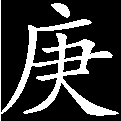
\includegraphics[width=3mm]{../Images/00004}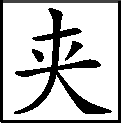
\includegraphics[width=3mm]{../Images/00012}\footnotesize \kaishu 偏{(立)}{[}写{]}贾政戏谑,已是异文,而贾环作诗实奇中又奇之奇文也,总在人意料之外。竟有人曰:``贾环如何又有好诗,似前言不搭后文矣。''盖不可向说问。贾环亦荣公{(子)}{[}之{]}正脉,虽少年顽劣,见今古小儿之常情耳。读书岂无长进之理哉?况贾政之教是弟子,自已大觉疏忽矣。若是贾环连一平仄也不知,岂荣府是寻常膏粱不知诗书之家哉?然后知宝玉之一种情思,正非有益之聪明,不得谓比诸人皆妙者也。}贾政看了,亦觉罕异,只是词句终带着不乐读书之意,遂不悦道:``可见是弟兄了。发言吐气总属邪派,将来都是不由规矩准绳,一起下流货。妙在古人中有`二难',你两个也可以称`二难'了。只是你两个的`难'字,却是作难以教训之`难'字讲才好。哥哥是公然以温飞卿自居,如今兄弟又自为曹唐再世了。''说的贾赦等都笑了。贾赦乃要诗瞧了一遍,连声赞好,道:``这诗据我看甚是有气骨。想来咱们这样人家,原不比那起寒酸,定要`雪窗萤火',一日蟾宫折桂,方得扬眉吐气。\elegantpar{咱们的子弟都原该读些书,不过比别人略明白些,可以做得官时就跑不了一个官的。何必多费了工夫,反弄出书呆子来。所以我爱他这诗,竟不失咱们侯门的气概。}{世卿世禄}''因回头吩咐人去取了自己的许多玩物来赏赐与他。因又拍着贾环的头,笑道:``以后就这么做去,方是咱们的口气,将来这世袭的前程定跑不了你袭呢。''贾政听说,忙劝说:``不过他胡诌如此,那里就论到后事了。''说着便斟上酒,又行了一回令。{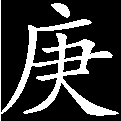
\includegraphics[width=3mm]{../Images/00004}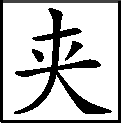
\includegraphics[width=3mm]{../Images/00012}\footnotesize \kaishu 便又轻轻抹去也。}贾母便说:``你们去罢。自然外头还有相公们候着,也不可轻忽了他们。况且二更多了,你们散了,再让我们姑娘们多乐一回,好歇着了。''贾赦等听了,方止了令,又大家公进了一杯酒,方带着子侄们出去了。要知端详,再听下回。

{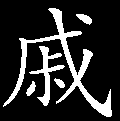
\includegraphics[width=3mm]{../Images/00005}\kaishu 总评:下回有一篇极清雅文字,下幅有半篇极整齐文字,故先叙抢快摸牌,沉湎酒色为反振,有骏马下坡、鸷鸟将翔之势。}

{\kaishu 看聚赌一段,宛然``宵小群居终日图'',看赏月一段,又宛然``望族序齿燕毛录'',说火则热,而说冰则寒,文心故无所不可。}

% {\href{../Text/part0079_split_000.html\#navto_1_a}{①}``谓'',原作``来'',疑在传抄过程中,``谓''音讹为``未'',``未''又再形讹为``来''。南唐画家徐熙所作花木禽鸟,``没骨渍染,轻淡野逸'',人称``落墨法''。{}}

% {\href{../Text/part0079_split_000.html\#navto_2_a}{②}``欹'',原作``歌'',诸本则作``倚''。按``欹''可能形讹为``歌'',或被改为``倚'',而``倚''则不致被误为``歌'',径改。(云涛说)}

% {\href{../Text/part0079_split_000.html\#navto_3_a}{③}此眉批与底本原抄字迹不同,当为后人所批。但也有人认为是原批,且``似是作者之长辈的语气''。姑存之。}{}
